\section{Results analysis}

\subsection{Overview}

This sections aims at describing the results observed when running the MEDEAS model integrating the created surrogate model, and comparing them with the results previously obtained with MEDEAS.

This comparison has to be made over the different scenarios that are defined in MEDEAS, that differ by the evolution of the electricity production mix. These scenarios were detailed in Section \ref{section:medeas-scenarios}. To streamline the analysis, we will focus on two scenarios: Busines As Usual (BAU) and Optimal Level Transision (OLT). The Mid-Level Transition scenario (MLT), falling between the two, does not contribute significantly to gaining valuable insights.

\subsection{Electricity production}

The purpose of this comparison is to highlight the impact of integrating the Dispa-SET surrogate model on electricity production values between two scenarios: the default MEDEAS runs and the modified MEDEAS runs integrating the Dispa-SET model.

To make this comparison, four runs are needed, default MEDEAS and modified MEDEAS, integrating the Dispa-SET surrogate model, both with BAU and OLT scenarios.

\subsubsection{Photovoltaic units}

The photovoltaic electricity production predictions from the four simulations are displayed in Figure \ref{fig:electricity-production-PV}.

\begin{figure}[h]
    \centering
    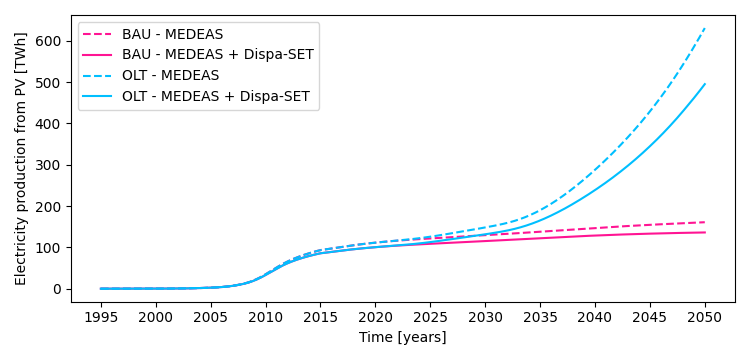
\includegraphics[width=0.8\textwidth]{resources/images/electricity-production_PV.png}
    \caption{Electricity production predictions from photovoltaic units}
    \label{fig:electricity-production-PV}
\end{figure}

We can observe that the modified MEDEAS predicts a lower amount of PV energy relatively to default MEDEAS, for both scenarios. In OLT, the difference becomes more pronounced as the production level rises, resembling the effect of linear scaling.

\subsubsection{Onshore wind}

Figure \ref{fig:electricity-production-onshore} illustrates the varying predictions of the onshore wind production.

\begin{figure}[h]
    \centering
    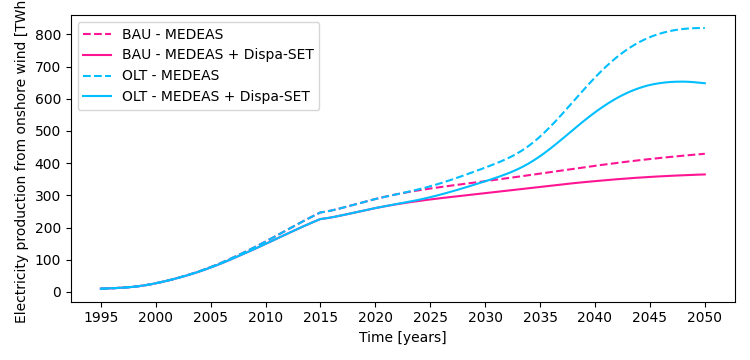
\includegraphics[width=0.8\textwidth]{resources/images/electricity-production-onshore.png}
    \caption{Electricity production predictions from onshore wind units}
    \label{fig:electricity-production-onshore}
\end{figure}

In a similar fashion to the PV production, the modified MEDEAS outputs what looks like a scaled version of the default MEDEAS output. Interestingly, a maximum is observed around 2050 in the OLT scenario with default MEDEAS. In contrast, this maximum is slightly shifted to around 2047 when utilizing the modified MEDEAS. 

\subsubsection{Offshore wind}

Predictions of the offshore wind electricity production in the four scenarios considered are given in Figure \ref{fig:electricity-production-offshore}.

\begin{figure}[h]
    \centering
    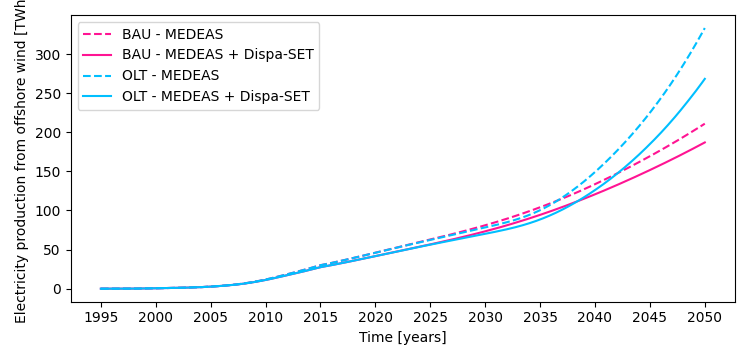
\includegraphics[width=0.8\textwidth]{resources/images/electricity-production-offshore.png}
    \caption{Electricity production predictions from offshore wind units}
    \label{fig:electricity-production-offshore}
\end{figure}

Offshore wind electricity results follows the trend observed previously, that is, the modified model predicting a smaller amount of electricity and overall as well as a larger production decrease in OLT.

\subsubsection{Hydroelectricity}

The results for hydroelectricity production across the four scenarios are depicted in Figure \ref{fig:electricity-production-hydro}.

\begin{figure}[h]
    \centering
    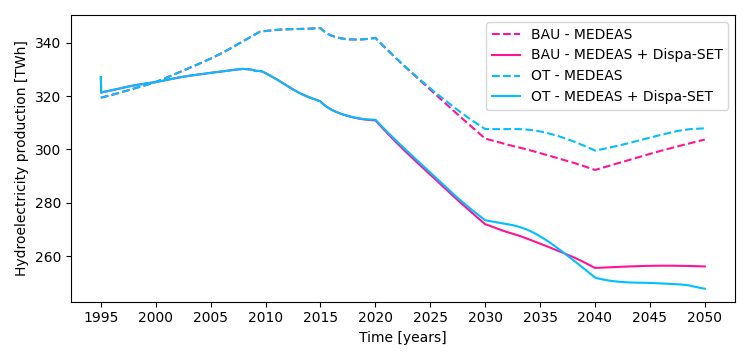
\includegraphics[width=0.8\textwidth]{resources/images/electricity-production-hydro.png}
    \caption{Electricity production predictions from hydroelectric units}
    \label{fig:electricity-production-hydro}
\end{figure}

Contrary to the previous results, where the results are grouped by scenario, that is, the shape of the curve is dictated by the scenario then is slightly changed by the model, these outcomes are grouped by model. In contrast, the outputs of the modified MEDEAS model for both the BAU and OLT scenarios are closely aligned with each other but distinctly diverge from the outputs of the default MEDEAS model.

This phenomenon can be explained by the fact that hydroelectricity is not favored by Dispa-SET, therefore these units are avoided when possible, hence leading to a smaller use. This may be due to the geographical constraints these units are suject to, limiting their growth are there is no spot to build new units.

These are also linked to pumped hydro-storage units, as there may be such a unit build on a river. On average, the unit produces the amount of electricty dictated by the river's flow, but the total energy produced over a set period is dependent on the specific dispatch of that unit, used as a tool to manoeuvre the electricity network.

\subsubsection{Electricity mix}

Figure \ref{fig:electricity-mixes} exhibits the different predictions for the electricity mix in 2050.

\begin{figure}[h]
    \centering
    \begin{subfigure}{0.34\textwidth}
        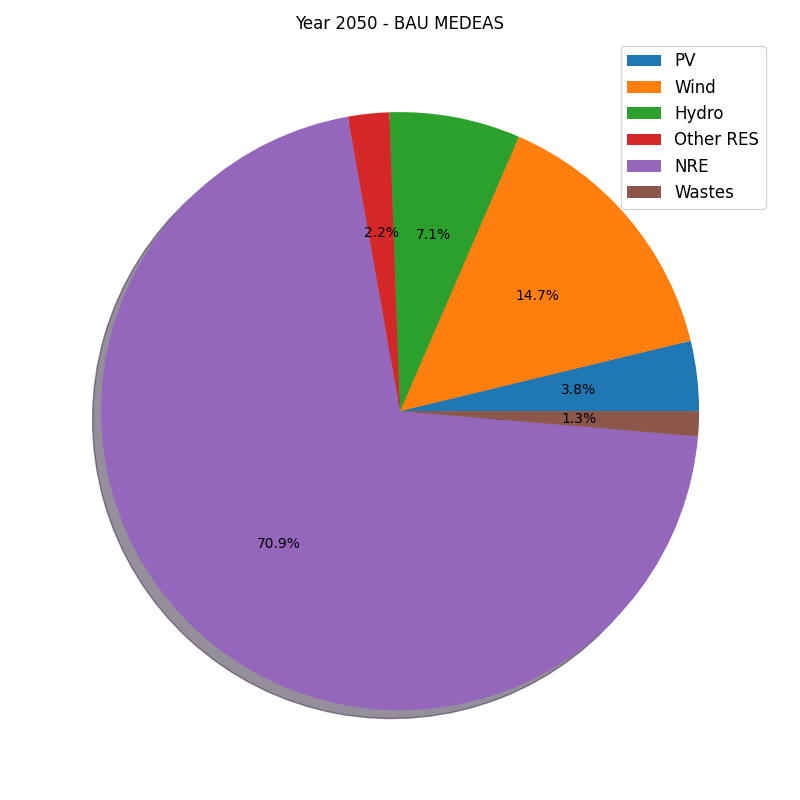
\includegraphics[width=\textwidth]{resources/images/electricity-mix-BAU-default.png}
        \caption{BAU using default MEDEAS}
        \label{fig:electricity-mix-BAU-def}
    \end{subfigure}
    \begin{subfigure}{0.34\textwidth}
        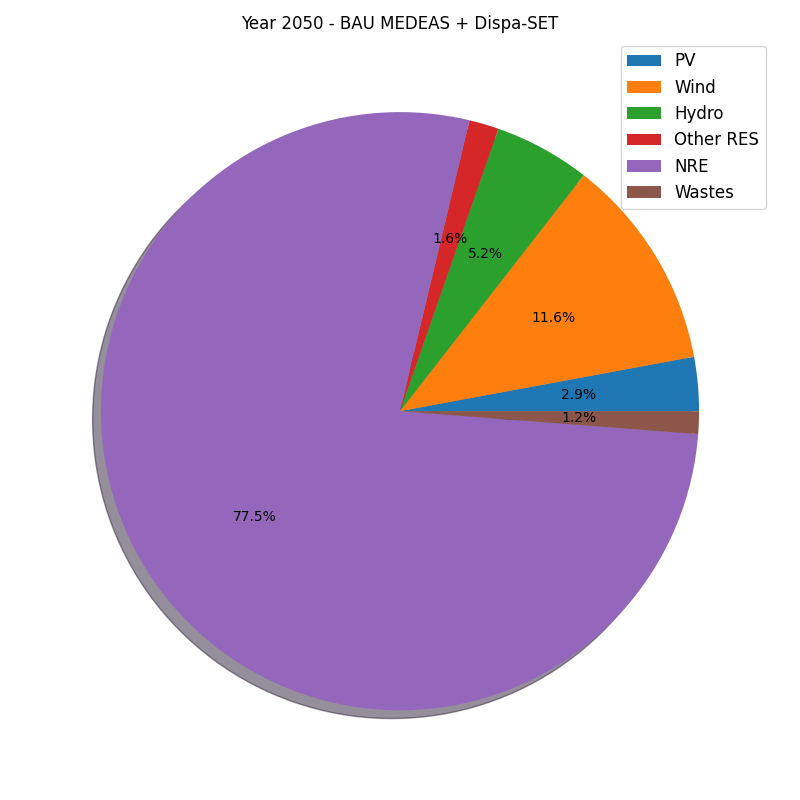
\includegraphics[width=\textwidth]{resources/images/electricity-mix-BAU-dispa.png}
        \caption{BAU using modified MEDEAS}
        \label{fig:electricity-mix-BAU-dispa}
    \end{subfigure}
    \hfill
    \begin{subfigure}{0.34\textwidth}
        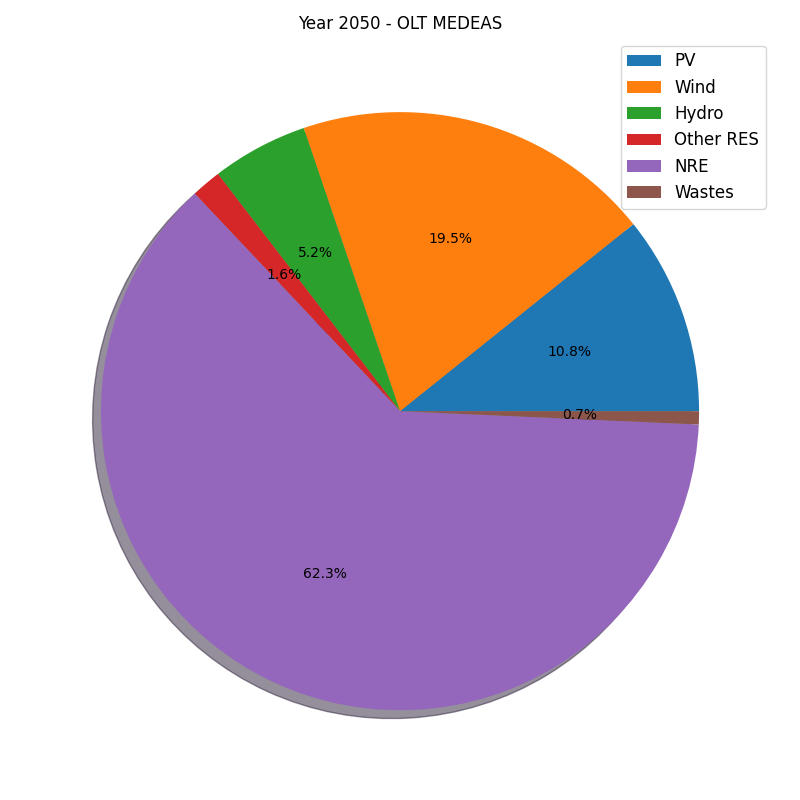
\includegraphics[width=\textwidth]{resources/images/electricity-mix-OLT-default.png}
        \caption{OLT using default MEDEAS}
        \label{fig:electricity-mix-OLT-def}
    \end{subfigure}
    \begin{subfigure}{0.34\textwidth}
        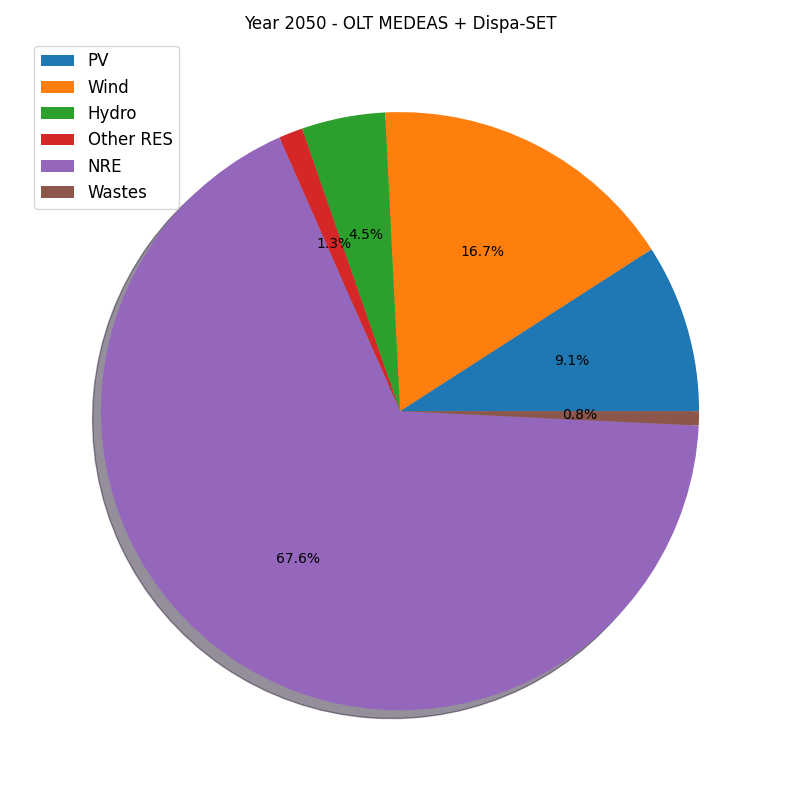
\includegraphics[width=\textwidth]{resources/images/electricity-mix-OLT-dispa.png}
        \caption{OLT using modified MEDEAS}
        \label{fig:electricity-mix-OLT-dispa}
    \end{subfigure}
    \caption{Electricity mix projection in 2050 for the four considered cases}
    \label{fig:electricity-mixes}
\end{figure}

Similar to the earlier observation revealing reduced VRES production, the proportion of VRES in the overall electricity mix is also lower in the modified version of the MEDEAS model.

A noteworthy change is the decrease in the share of hydroelectricity in the OLT scenario compared to the BAU scenario, for both default and modified MEDEAS. This can likely be attributed to the overall higher total production in the OLT scenario, leading to a relatively diminished share as hydroelectricity generation remains constant.
% The most intriguing change is the lower share of hydroelectricity in OLT compared to BAU, for both default and modified MEDEAS. The most likely cause for this that the total production is larger, hence as there is no growth in hydroelectricity generation, the share is reduced. 

\subsection{Curtailment}

As the surrogate model explicitly outputs the curtailment, this variable can then be plotted over a run of the modified MEDEAS. The results obtained for both scenarios are displayed in Figure \ref{fig:electricity-production-curtailed}.

\begin{figure}[h]
    \centering
    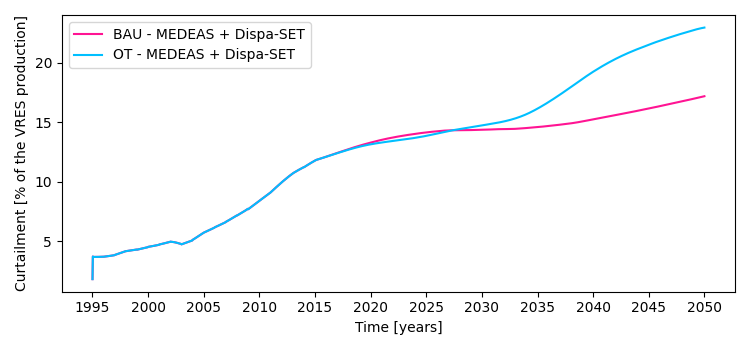
\includegraphics[width=0.9\textwidth]{resources/images/electricity-production-curtailed.png}
    \caption{Curtailment prediction of the modified MEDEAS for BAU and OLT scenarios}
    \label{fig:electricity-production-curtailed}
\end{figure}

We can observe from Figure \ref{fig:electricity-production-curtailed} that the OLT scenarios suffers from higher proportions of curtailment, with an higher growth rate, than in the BAU scenario. However, this increase rate looks stable.

It may be concluded that curtailment is inevitable, nonetheless every option has not been covered. For example, the distinction between different types of storage units based on the storage capacity to power output ratio has not been made. As storage facilities have a massive influence on curtailment, a more accurate modelling of these may be insightful.

\subsection{Discussion}

The figures presented consistently conclude that integrating the surrogate model, i.e. taking power systems constraints into account, leads to a lower prediction of electricity production from VRES. This outcome is somewhat counterintuitive, as the consideration of the increasing part of curtailment suggest larger amounts of wasted energy.

A plausible interpretation matching the observations is that due to the more restrictive constraints, the deployment of VRES is more challenging than previously estimated. Hence, as more efforts are required to achieve the same share of renewable energy production, e.g. because a storage unit has to be built as well, the same amount of effort yields a lower VRES share.


% Tools have been made to automate the creation of a dataset, including sampling and running the model; and the training of the surrogate model, using machine learning methods. The integration of the model into Vensim 